\documentclass[12pt]{article}
\usepackage[top=1in, bottom=1in, left=.75in, right=.75in]{geometry}
\usepackage{amsmath}
\usepackage{fancyhdr}
\usepackage{graphicx}
\usepackage{txfonts}
\usepackage{multicol}
\usepackage[scaled=0.86]{helvet}
\renewcommand{\emph}[1]{\textsf{\textbf{#1}}}
\usepackage{anyfontsize}
% \usepackage{times}
% \usepackage[lf]{MinionPro}
\usepackage{tikz,pgfplots}
%\def\degC{{}^\circ{\rm C}}
\def\ra{\rightarrow}
\usetikzlibrary{calc}
\pgfplotsset{compat = newest}
\newcommand{\blank}[1]{\rule{#1}{0.75pt}}

\pgfplotsset{my style/.append style={axis x line=middle, axis y line=
middle, xlabel={$x$}, ylabel={$y$},axis equal}}

%yticklabels={,,} , xticklabels={,,}

% \setmainfont{Times}
% \def\sansfont{Lucida Grande Bold}
\parindent 0pt
\parskip 4pt
\pagestyle{fancy}
\fancyfoot[C]{\emph{\thepage}}
\fancyhead[L]{\ifnum \value{page} > 1\relax\emph{Math 251: Midterm 1}\fi}
\fancyhead[R]{\ifnum \value{page} > 1\relax\emph{September 23, 2021}\fi}
\headheight 15pt
\renewcommand{\headrulewidth}{0pt}
\renewcommand{\footrulewidth}{0pt}
\let\ds\displaystyle
\def\continued{{\emph {Continued....}}}
\def\continuing{{\emph {Problem \arabic{probcount} continued....}}\par\vskip 4pt}


\newcounter{probcount}
\newcounter{subprobcount}
\newcommand{\thesubproblem}{\emph{\alph{subprobcount}.}}
\def\problem#1{\setcounter{subprobcount}{0}%
\addtocounter{probcount}{1}{\emph{\arabic{probcount}.\hskip 1em(#1)}}\par}
\def\subproblem#1{\par\hangindent=1em\hangafter=0{%
\addtocounter{subprobcount}{1}\thesubproblem\emph{#1}\hskip 1em}}
\def\probskip{\vskip 10pt}
\def\medprobskip{\vskip 2in}
\def\subprobskip{\vskip 45pt}
\def\bigprobskip{\vskip 4in}

\begin{document}
{\emph{\fontsize{26}{28}\selectfont Math F251\hfill
{\fontsize{32}{36}\selectfont Midterm 1}
\hfill Fall 2021}}
\vskip 2cm
\strut\vtop{\halign{\emph#\hskip 0.5em\hfil&#\hbox to 2in{\hrulefill}\cr
\emph{\fontsize{18}{22}\selectfont Name:}&\cr
\noalign{\vskip 10pt}
%\emph{\fontsize{18}{22}\selectfont Student Id:}&\cr
%\noalign{\vskip 10pt}
%\emph{\fontsize{18}{22}\selectfont Calculator Model:}&\cr
}}
\hfill
\vtop{\halign{\emph{\fontsize{18}{22}\selectfont #}\hfil& \emph{\fontsize{18}{22}\selectfont\hskip 0.5ex $\square$ #}\hfil\cr
Section: & F01 (Jill Faudree)\cr
\noalign{\vskip 4pt}
         & F02 (James Gossell)\cr
\noalign{\vskip 4pt}
         & UX1 (James Gossell)\cr}}

\vfill
{\fontsize{18}{22}\selectfont\emph{Rules:}}

You have 60 minutes to complete the exam.  

Partial credit will be awarded, but you must show your work.

The exam is closed book and closed notes.

Calculators are not allowed. 


Place a box around your  \fbox{FINAL ANSWER} to each question where appropriate.

If you need extra space, you can use the back sides of the pages.
Please make it obvious  when you have done so.

Turn off anything that might go beep during the exam.

Good luck!
\vfill
\def\emptybox{\hbox to 2em{\vrule height 16pt depth 8pt width 0pt\hfil}}
\def\tline{\noalign{\hrule}}
\centerline{\vbox{\offinterlineskip
{
\bf\sf\fontsize{18pt}{22pt}\selectfont
\hrule
\halign{
\vrule#&\strut\quad\hfil#\hfil\quad&\vrule#&\quad\hfil#\hfil\quad
&\vrule#&\quad\hfil#\hfil\quad&\vrule#\cr
height 3pt&\omit&&\omit&&\omit&\cr
&Problem&&Possible&&Score&\cr\tline
height 3pt&\omit&&\omit&&\omit&\cr
&1&&10&&\emptybox&\cr\tline
&2&&8&&\emptybox&\cr\tline
&3&&12&&\emptybox&\cr\tline
&4&&10&&\emptybox&\cr\tline
&5&&20&&\emptybox&\cr\tline
&6&&12&&\emptybox&\cr\tline
&7&&8&&\emptybox&\cr\tline
&8&&6&&\emptybox&\cr\tline
&9&&14&&\emptybox&\cr\tline
&Extra Credit&&3&&\emptybox&\cr\tline
&Total&&100&&\emptybox&\cr
}\hrule}}}

\newpage
\begin{enumerate}
%%%PAGE 1
%%%%LIMITS + DERIVATIVES FROM GRAPHs
\item{10 points} The graph of the function $f(x)$ is given below. The domain of $f(x)$ is $(-\infty,\infty).$ 
Determine the following. If the value does not exist, write ``DNE''.
%%%%FIGURE
\begin{center}
 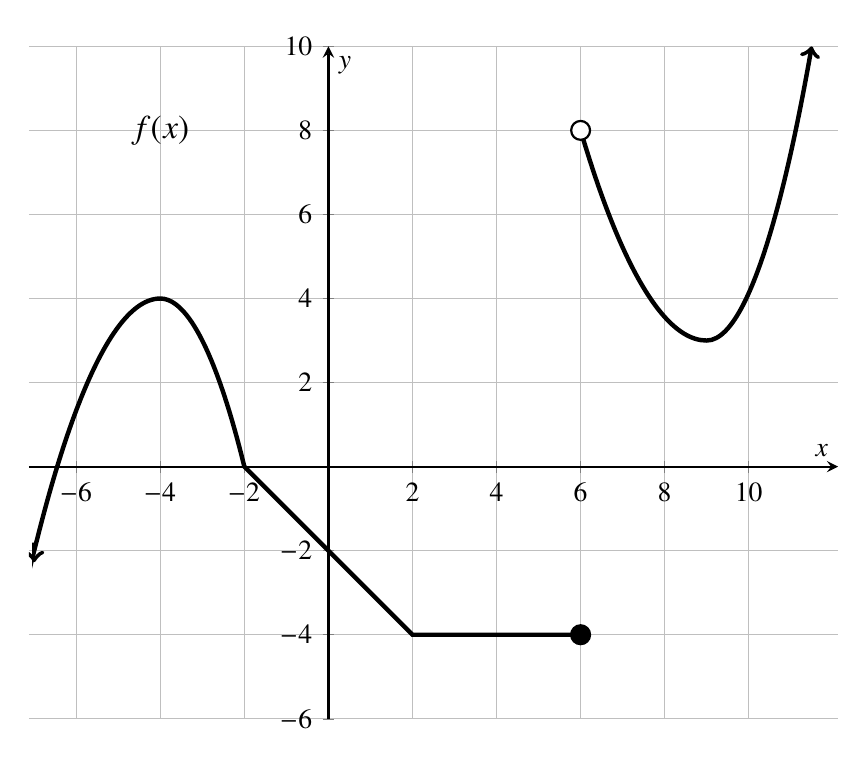
\begin{tikzpicture}
\begin{axis}[x=1cm,y=1cm,scale=1.5,xscale=1, thick, my style, xtick={-6,-4,...,10}, ytick={-6,-4,...,10},xmin=-6, xmax=11, ymin=-6, ymax=10, 
mark size=3.0pt, grid = major]
\addplot[ultra thick,>-] (-7, -2) parabola bend (-4,4)  (-2,0) to  (2,-4) to (6,-4);
\addplot[ultra thick,->] (6, 8) parabola bend (9,3)  (11.5,10);
\node at (-4,8){\large{$f(x)$}};
\draw[fill=black, thick] (6,-4) circle  (1.2 mm);
\draw[fill=white, thick] (6,8) circle  (1.2 mm);
\end{axis}
\end{tikzpicture}\end{center}

\newcommand{\ans}{\rule{1.5cm}{.5 pt}}
\newlength{\mysep} 
\setlength{\mysep}{0.3in}
%%%%%QUESTIONS
\begin{enumerate}
\begin{multicols}{2}
\item $f(6) = \ans$
\bigskip

\item $\displaystyle{\lim_{x\to 6^{+}} f(x) }= \ans$
\bigskip

\item $ \displaystyle{ \lim_{x\to 6^-} f(x) }= \ans$
\bigskip

\item $ \displaystyle{ \lim_{x\to 6} f(x) }= \ans$
\bigskip



\item $\displaystyle{ \lim_{x \to -4} f(x) }= \ans$
\bigskip

\item $\large{f'(0)}= \: \ans $
\bigskip

\vspace{\mysep}
\end{multicols}
\vspace{1cm}
\item List the $x$-values where $f(x)$ fails to be continuous.\\
\vfill
\item List the $x$-values for which $f(x)$ fails to have a derivative.\\\vfill
\vspace{\mysep}
\end{enumerate}
\newpage
%%%%PAGE 2
%%%%SYMBOLIC DERIVATIVES
\item (8 points) Suppose that $f$ and $g$ are differentiable functions with $f(2)=6$, $f'(2)=1$, $g(2)=5$, and $g'(2)=2$. For $h(x)=f(x)\cdot g(x)$ and $k(x)=\large{\displaystyle{\frac{f(x)}{g(x)}}}$, evaluate the following derivatives:\\ 

	\begin{enumerate}

	\item $h'(2)=$\\ \vfill

	\item $k'(2)=$\\ \vfill 

	\end{enumerate}

%%%%%%%%APPLIED EXPLANATION
\item (12 points) A company's profit in thousands of dollars when $x$ units are produced is given by $$P(x)=-0.001x^2+0.22x-42.$$

	\begin{enumerate}

	\item Observe that $P(1200) = 78$. Interpret this fact in the context of the problem. To earn full credit your answer should be a complete sentence and must include units.

	\vspace{1in}

	\item Observe that $P'(1200) = -0.02$. Interpret this fact in the context of the problem. To earn full credit your answer should be a complete sentence and must include units.

	\vspace{1in}

	\item Suppose the company is currently producing 1200 units. Should the company increase production if it wants to increase profits? \textbf{Justify} your answer.
\vfill
	\end{enumerate}
\newpage

%%%%PAGE 3
%%%%%DEFINTION OF DERIVATIVE
\item (10 points) Find the derivative of $f(x)=\large{\displaystyle{\frac{4}{x+1}}}$ \textbf{using the definition of the derivative}. No credit will be awarded for using another method.
\newpage
%%%%%%%PAGE 4
%%%%%%%ASSORTMENT OF LIMITS
\item (20 points) Evaluate the following limits. Give the most complete answer; if the limit is infinite, indicate that with $\infty$ or $-\infty.$ If a value does not exist, write DNE.\\
	\begin{enumerate}
	\item $\displaystyle{\lim_{x  \to 5} \frac{5x-x^2}{20+x-x^2}=}$
	\vfill
	\item $\displaystyle{\lim_{x \to 7^+ }  \frac{x+12}{7-x}=}$
	\vfill
	\item $\displaystyle{\lim_{h \to 0 } \frac{\sqrt{x+h} -\sqrt{x}}{h} =}$
	\vfill
	\item $\displaystyle{\lim_{t \to 0^-} \left(\frac{t}{2} + \frac{6}{t-2} \right)=}$
	\vfill
	\end{enumerate}
\newpage
%%%%PAGE 5
%%%%%%%% STRAIGHT DERIVATIVES
\item (12 points) Find $f'(x)$ for each of the following expressions. You do not need to simplify.

	\begin{enumerate}

	\item $f(x)=6x^3+5x^2-\sqrt{x}+\sqrt{\pi}$\\ \vfill

	\item $f(x)=\frac{2x-4}{x^2+1}$\\ \vfill

\end{enumerate}
%%%%SKETCH DERIVATIVE FROM GRAPH OF FUNCTION
\item (8 points) The graph of $g(x)$ is graphed below. Sketch the graph of its derivative $g'(x)$.

\begin{center}
 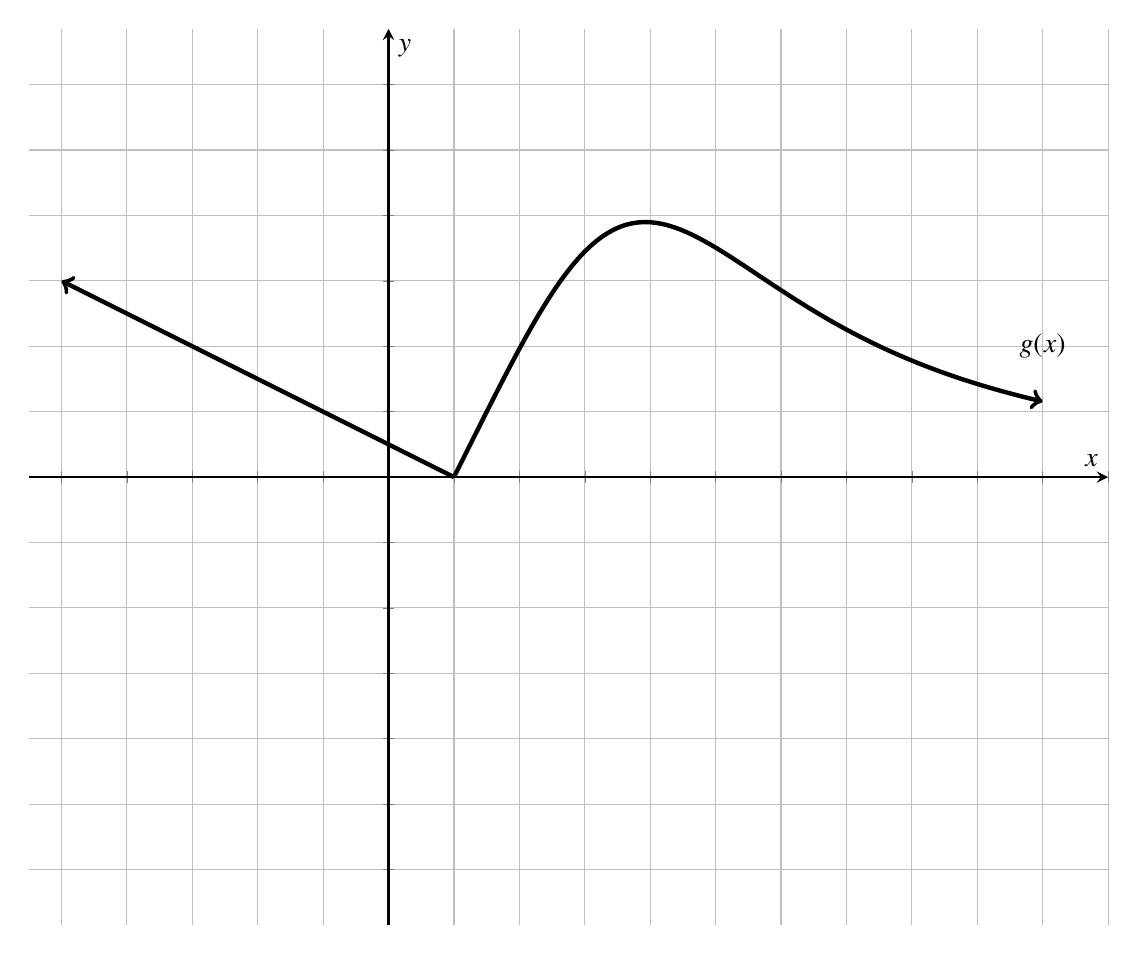
\begin{tikzpicture}
\begin{axis}[scale=2,xscale=1, thick, my style, xtick={-5,-4,...,11}, ytick={-6,-5,...,6},xmin=-5.5, xmax=11, ymin=-6, ymax=6, 
mark size=3.0pt, grid = major,yticklabels={,,} , xticklabels={,,}]
\addplot[ultra thick, ->,domain=1:10, samples=100]{100*(x-1)/((x-1)*(x-1)*(x-1)+50)};
\addplot[ultra thick, <-,domain=-5:1, samples=100]{-x/2+0.5};
\node at (10,2){$g(x)$};
\end{axis}
\end{tikzpicture}\end{center}

\newpage
%%%%%PAGE 6
%%% slope of tangent
\item (6 points) The questions below reference the function $f(x)=(3-x)(x-7).$ 
	\begin{enumerate}
	\item Find the slope of the line tangent to at $x=4$. 
	\vfill
	
	\item Sketch the tangent line to $f(x)$ at $x=4$ on the graph of $f(x)$ below.

\begin{center}
 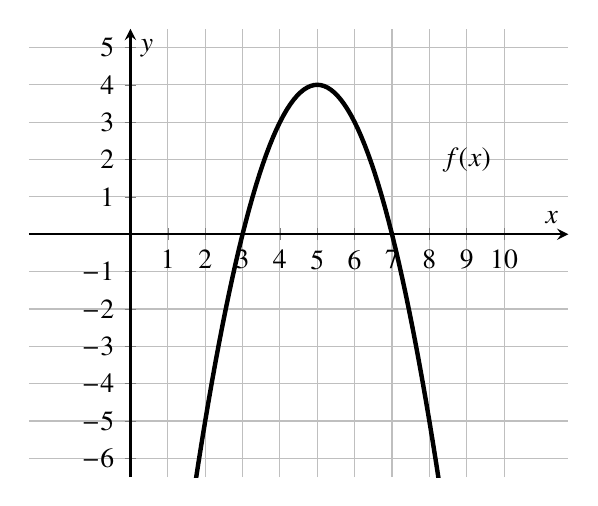
\begin{tikzpicture}
%quadratic
\begin{axis}[scale=1,xscale=1, thick, my style, xtick={0,1,...,10}, ytick={-6,-5,...,5},xmin=-0.5, xmax=9.5, ymin=-6.5, ymax=5.5, 
mark size=3.0pt, grid = major]
\addplot[ultra thick, <->,domain=0:9, samples=100]{(3-x)*(x-7)};
%\addplot[ultra thick, <-,domain=-6:0, samples=100]{-x};
\node at (9,2){$f(x)$};
\end{axis}
\end{tikzpicture}\end{center}
\end{enumerate}
%%%%velocity and acceleration
\item (14 points) Patrick throws a football straight up from the surface of the moon. While the football is in the air, its height in meters after $t$ seconds is $h(t)=t(16-0.8t)$. Answer the following questions {\bf including units in your answers}.

	\begin{enumerate}

	\item What is the initial velocity of the football?\\ \vfill

	\item When will the football reach its highest point?\\ \vfill

	%\item How high will the football go?\\ \vfill

	\item When will the football hit the ground?\\ \vfill

	\item What is the acceleration due to gravity on the moon?\\ \vfill

\end{enumerate}
\newpage
\item \textbf{Extra Credit} (3 points)Use the Intermediate Value Theorem to \textbf{prove} that there exists some
$x$-value in the interval $(0,100)$ such that the function $g(x)=e^{-x}+\sqrt{x}+8$ takes the value $y=10.$ Full credit will only be given if the solutions provides and explanation using complete sentences.

\end{enumerate}
\end{document}












\vspace{1in}




\newpage
\problem{extra credit} Use the Intermediate Value Theorem to prove that there exists some
$x$-value in the interval $(0,100)$ such that the function $g(x)=e^{-x}+\sqrt{x}+8$ takes the value $y=10.$



\end{document}


%%%%%%%%%END
\problem{10 points}

In the diagram below, sketch the graph
of a function  $f(x)$ defined on all the real numbers
satisfying the following criteria.
 
% \begin{multicols}{3}
    \begin{enumerate}
        \item $\ds \lim_{x\to 2}f(x)=1$
        \item $f(x)$ is not continuous at $x=1$
        \item $\ds \lim_{x\to 4-}f(x)=\infty$
        \item $\ds f(4)=-1$
        \item $\ds \lim_{x\to \infty}f(x)=0$
        \item $\ds \lim_{x\to 0^+}=-1$
        \item $\ds \lim_{x\to 0^-}=2$
        \item $\ds f(-2)=-1$
        \item $\ds f(x)$ is a linear function on $[-2,0]$
    \end{enumerate}
% \end{multicols}
\vfill
\begin{center}
\begin{tikzpicture}[xscale=1.5,yscale=1.5]
\draw [help lines,dashed] (-3,-3) grid (6.2,3.2);
\draw [thick, ->] (-3,0)--(6.2,0) node[right] {$x$};
\draw [thick, ->] (0,-3)--(0,3.2) node[above]{$f(x)$};
\foreach \i in {-2,2,4}
{       \node[below] at (\i,0) {$\i$};
}
\foreach \i in {-2,2}
{       \node[left] at (0,\i) {$\i$};
}
\end{tikzpicture}
\end{center}
\vfill
\newpage
\problem{10 points} For a particular function $f(x)$,
\[
f(1)=4,\quad f(4)=1,\quad f'(1)=0\quad\text{and}\quad f'(4)=2.
\]
\subproblem{} Find the equation of the tangent line
of the graph of $f(x)$ at $x=4$.
\vfill
\subproblem{}
\begin{itemize}
	\item On the axes below make a rough sketch of what the graph $y=f(x)$ might look like, using all of the limited information that you have.
	\item Sketch the tangent line at $x=1$.
	\item Sketch the tangent line at $x=4$.
\end{itemize}

\hfil\begin{tikzpicture}[xscale=2.5,yscale=1.5]
\draw [help lines,dashed] (0,-2) grid (5.2,5.2);
\draw [thick, ->] (0,0)--(5.2,0) node[right] {$x$};
\draw [thick, ->] (0,-2)--(0,5.2) node[above]{$f(x)$};
\foreach \i in {2,4}
{       \node[below] at (\i,0) {$\i$};
}
\foreach \i in {2,4}
{       \node[left] at (0,\i) {$\i$};
}
\end{tikzpicture}


\newpage

\problem{16 points}  Compute, with justification, the following limits, or explain why the given limit does not exist. 
\begin{itemize}
\item \textbf{Use proper limit notation for full credit.}
\item  If a limit is \textbf{positive or negative infinity}, state that explicitly and justify your answer \textbf{without using a sketch}.
\end{itemize}
\vskip 12pt

\subproblem{}$\ds\lim_{h\to 0} \frac{\sqrt{9+h}-3}{h}$
\vfill
\continued
\newpage
\continuing
\vskip 12pt

\subproblem{} $\ds\lim_{x\to 5^+} \frac{x^2-3x}{5-x}$
\vfill
\subproblem{} $\ds\lim_{x\to\infty} \frac{\sqrt{5x^2-2}}{3-2x}$
\vfill
\subproblem{} $\ds\lim_{x\to\infty} \sin\left(\frac{\sqrt{5x^2-2}}{3-2x}\right)$
\vskip 1cm
\newpage
\problem {10 points}  An icicle is growing
at the back of a house.  At time $t\ge 0$
days the length of the icicle is
$$
\ell(t) = \frac{14 t + 4}{t+2}
$$
inches.  Answer the following questions about the
function $\ell(t)$ and be sure to include \textbf{units}
in your answers.

\subproblem{} Compute the average rate of change of
the length of the icicle from time $t=0$ to time $t=2$
days.  \textbf{Do not forget units!}
\vfill

\subproblem{}  It is a known fact that $\ds \ell'(t) = \frac{24}{(t+2)^2}$.
Compute $\ell'(2)$ (\textbf{with units}) and explain what this quantity 
means about the icicle.
\vfill

\subproblem{}
Compute $\lim_{t\to\infty} \ell(t)$.
Then explain what this quantity means in precise
but everyday language that the general public would understand. 
Do not forget units!
\vfill
\newpage
\problem{10 points}
Use the \textbf{definition of the derivative} to compute
$f'(2)$ if $f(x)=7x^2$. No credit will be given if a different method is used.

\newpage
\problem{8 points}

Match the graph of each function (a) - (d) with the
graph of its derivative I-IX. Write your answers in the blanks
provided below.\medskip

\halign{#&\qquad#\cr
1. The derivative of graph (a) is \blank{1in} & 3. The derivative of graph (b) is \blank{1in}\cr
\noalign{\vskip 8pt}
2. The derivative of graph (c) is \blank{1in} & 4. The derivative of graph (d) is \blank{1in}\cr}\par\bigskip

\hrule
\emph{Functions:}
\begin{center}
 \begin{tabular}{llcll}
a)&\includegraphics{Graphics/MT1-matching-quartic}
&\qquad&b)&\includegraphics{Graphics/MT1-matching-atan}\\
&&&&\vspace{.4in}\\
c)&\includegraphics{Graphics/MT1-matching-sqrt}&\qquad&d)&\includegraphics{Graphics/MT1-matching-cubic}
\end{tabular} 
\end{center}

\smallskip
\hrule
\emph{Derivatives:}

\begin{center}
%%Version 1
\begin{tabular}{llcllcll}
I.&\includegraphics{Graphics/MT1-matching-quartic-prime-fake}&\qquad&
II.&\includegraphics{Graphics/MT1-matching-sqrt-prime}&\qquad&
III.&\includegraphics{Graphics/MT1-matching-atan-prime-fake}\\
&&&&\vspace{.3in}\\
IV.&\includegraphics{Graphics/MT1-matching-quartic-prime}&\qquad&
V.&\includegraphics{Graphics/MT1-matching-cubic-prime-fake2}&\qquad&
VI.&\includegraphics{Graphics/MT1-matching-sqrt-prime-fake}\\
&&&&\vspace{.3in}\\
VII.&\includegraphics{Graphics/MT1-matching-cubic-prime-fake}&\qquad&
VIII.&\includegraphics{Graphics/MT1-matching-atan-prime}&\qquad&
IX.&\includegraphics{Graphics/MT1-matching-cubic-prime}
\end{tabular}\end{center}
\newpage


% \begin{axis}[scale=1, axis x line=middle, axis y line=
% middle, xlabel={$x$}, ylabel={$y$}, xtick={-4,-3,...,4}, ytick={-2,-1,...,4},
% xmin=-5, xmax=5, ymin=-3, ymax=5, minor y tick num=1,
%         minor x tick num=1, mark size=3.0pt]
% % \addplot[domain=-4.4:-3,<-,ultra thick] {0.1*((x+3)^2)+2};
% % \addplot[domain=-3:1, smooth, tension=1, ultra thick] coordinates { (-3,2) (-1,1.8) (0,1) (1,0)};
% % \addplot[domain=1:3.8, ultra thick,->] {(x-4)^(-1)+3.3};
% % \addplot[domain=4.2:5,<->, ultra thick]{(x-4)^(-1)};
% % \addplot[dashed,<->] coordinates {(4,4.5) (4,-2)};
% % \addplot[mark=*,only marks] coordinates {(-3,1)(1,0)};
% % \addplot[mark=*,fill=white,only marks] coordinates {(-3,2)(1,3)};
% \end{axis}
% \end{center}

\problem{Extra Credit: 3 points}
In problem \emph{3a} you computed the following limit:
\[
\lim_{h\to 0} \frac{\sqrt{9+h}-3}{h}.
\]
In fact, this limit is a computation, from the definition
of the derivative, of $f'(a)$ for some function $f(x)$
and some $x$-value $a$.  What is $f(x)$ and what is $a$?

\end{document}
